\chapter{Linear Algebra in a Nutshell}

This chapter gives an overview of linear algebra, including its scope and how the different terminologies and tools used in linear algebra are related to each other. The purpose of this chapter is to help the reader build the bird's-eye view and make them feel more under control when encountering the abstract concepts in later chapters.

Consider this chapter as additional help. Everything in this chapter will be formally introduced in later chapters at some point. The reader is free to skip this chapter should such help not required.

\section{Algebra}

The term ``algebra'' has a rich variety of meanings. In the context of elementary mathematics, \mync{algebra} may be viewed as a way of studying quantities and their relationships using symbols rather than specific numerical values. By introducing symbols, the focus shifts from solving a particular problem to discovering general principles that apply to many problems at once.

The following example illustrates this idea.

\begin{shortbox}
	\Boxhead{A Motivating Example of Algebra}
	
	Consider the problem of finding the area of an annulus whose outer radius is $2$ and whose inner radius is $1$.
	
\end{shortbox}

The area can be computed directly by subtracting the area of the smaller circle from that of the larger circle:
\begin{eqnarray}
	S &=& 2^2\pi - 1^2\pi \nonumber \\
	&=& 3\pi. \nonumber
\end{eqnarray}

Surprisingly, when I first encountered this problem as a primary school student, I arrived at a different approach. Imagine a line segment of length $2-1=1$ rotating about the centre of the annulus. As it rotates, it sweeps out the entire annular region, as illustrated in Fig.~\ref{fig:area-of-annulus}. The bold black segment represents the rotating line segment, while the shaded red region represents the area that has already been swept out.

\begin{figure}[!htb]
	\centering
	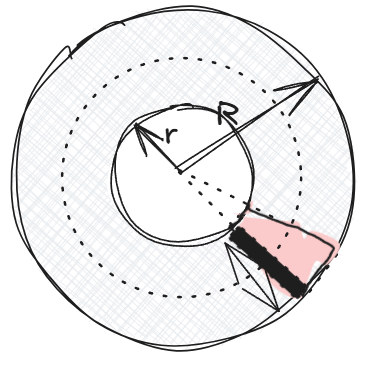
\includegraphics[width=0.6\textwidth]{chapters/part-1/figures/area_of_annulus.png}
	\caption{Calculating the area of an annulus by sweeping a line segment.}
	\label{fig:area-of-annulus}
\end{figure}

The total area swept out by the segment should therefore be equal to the length of the segment multiplied by the distance it travels. A similar idea is often used when explaining the area of a parallelogram, where a line segment sweeps out a region through horizontal or vertical translation.

The difficulty in the present problem is that the segment rotates rather than translates. During the rotation, its two endpoints travel along circles of different circumferences. It is therefore not immediately clear what distance should be used in the calculation. My intuition was that the appropriate distance should be the one traveled by the midpoint of the segment, which traces out the dashed circle shown in the figure. At the time, I had no proof that this choice was correct; it simply seemed the most natural one.

Using this idea, the area of the annulus is
\begin{eqnarray}
	S &=& (2-1)\times \left(\pi(2+1)\right) \nonumber \\
	&=& 3\pi, \nonumber
\end{eqnarray}
where $(2-1)$ is the length of the segment and $\pi(2+1)$ is the distance traveled by its midpoint given by the dashed circle in Figure \ref{fig:area-of-annulus}. Since $(2+1)$ is the diameter of the dashed circle, $\pi(2+1)$ is precisely its circumference. The result agrees with the direct calculation given earlier.

We want to know whether my method would always produce the correct answer for any annulus with a different pair of inner and outer radius. Looking back at the solution and with the more abstract and powerful tool of algebra, it can be done easily. Let $R$ and $r$ denote the outer and inner radius of the annulus respectively. Using the first approach, we obtain 
\begin{eqnarray} 
	S &=& \pi R^2 - \pi r^2. \nonumber 
	\end{eqnarray} 
Using the second approach, the length of the rotating segment is $R-r$, while the distance traveled by its midpoint is the circumference of a circle with diameter $R+r$. Hence, 
\begin{eqnarray} 
	S &=& (R-r)\pi(R+r) \nonumber \\ 
	&=& \pi(R^2-r^2) \nonumber \\ 
	&=& \pi R^2 - \pi r^2. \nonumber 
\end{eqnarray} 
The two approaches therefore give exactly the same result. 

More importantly, by replacing the specific numbers $2$ and $1$ with the symbols $R$ and $r$, we have transformed a particular arithmetic problem into a general statement. Instead of obtaining a result for only one annulus, we have derived a formula that applies to every annulus. The symbols allow us to identify the underlying relationship 
\begin{eqnarray} 
	R^2-r^2 = (R-r)(R+r), \nonumber 
\end{eqnarray} 
which explains why the two seemingly different methods lead to the same answer. 

This illustrates one of the central ideas of algebra. Rather than studying individual numerical examples, we use symbols to uncover general patterns and relationships that hold in a wide range of situations. By using the symbols, the problem becomes abstract to some extent, and in return we have a more generalized solution and more insightful understanding about the problem.

\section{Linear Algebra}

Linear algebra is a subset of algebra. It studies a particular portion of algebra that concerns with vector and linear transformation, both of which introduced in the next sections.

\subsection{Vector and Vector Space}

A vector is an element of a vector space. A vector space is an algebraic structure consisting of a non-empty set of objects, called vectors, together with two operations, vector addition and scalar multiplication. These operations satisfy a collection of axioms, commonly known as the vector space axioms. The abstract definition of a vector space belongs to the subject of abstract algebra and will be discussed in greater detail in Part II of this book.

For the moment, it is sufficient to think of a vector as an ordered list of real numbers of fixed length. Two operations can be performed on such vectors.

Vector addition. The sum of two vectors is obtained by adding their corresponding components. Let $x = [x_1,\ldots,x_n]^T$, $y = [y_1,\ldots,y_n]^T$. Their sum is given by
\begin{eqnarray}
	x+y
	&=&
	\left[
	\begin{array}{c}
		x_1+y_1 \\
		\vdots \\
		x_n+y_n
	\end{array}
	\right].
	\nonumber
\end{eqnarray}

Vector subtraction is defined similarly by subtracting corresponding components.

Scalar multiplication. Multiplying a vector by a scalar is done by multiplying each component by that scalar. Let $x = [x_1,\ldots,x_n]^T$ and let $c$ be a scalar. Then
\begin{eqnarray}
	cx
	&=&
	\left[
	\begin{array}{c}
		cx_1 \\
		\vdots \\
		cx_n
	\end{array}
	\right].
	\nonumber
\end{eqnarray}

At this stage, one may think of a vector space as a collection of vectors of the same dimension together with the operations of vector addition and scalar multiplication. This description captures the examples that will be studied in the first part of this book, although the formal definition introduced later is considerably more general.

Readers with a computer science or engineering background may find it helpful to think of vectors as a generalization of scalar numbers. A scalar may be regarded as a vector of dimension $1$. From this perspective, vector addition and scalar multiplication naturally extend the familiar arithmetic operations on real numbers.

Notice that a vector space, like any algebraic structure, must be closed to the operations defined on them. In the case of vector space, this would mean that if $V$ is a vector space, $\forall x, y \in V$, $x + y \in V$, and $\forall x \in V$, $cx \in V$. Examples of vector spaces include $\mathbb{R}^n$ and $\{[x_1,x_2]^T|x_1 = 2x_2\}$, etc. It can be easily proved that the above examples are all close with respect to vector addition and scalar multiplication. On the other hand, $\mathbb{Z}^n$ is not a vector space because it may be closed to scalar multiplications with $c$ a fraction. Similarly, $\mathbb{R}^n_{+}$ is not a vector space either, as it is not closed to scalar multiplications with negative $c$.

\subsection{Linear Transformation}

A \mync{transformation} is a mapping that takes an input and produces an output according to a specified rule. A \mync{linear transformation} is a transformation $T: V\to W$ between two vector spaces that preserves vector addition and scalar multiplication which is known as the \mync{superposition principle of linear system}. That means for all  $v,v_1,v_2\in V$ and scalar $c$,
\begin{eqnarray}
	T(v_1+v_2)
	&=&
	T(v_1)+T(v_2),
	\nonumber \\
	T(cv)
	&=&
	cT(v).
	\nonumber
\end{eqnarray}
Superposition principle of linear system implies that a linear transformation preserves the linear structure of a vector space.

An example of linear transformation is given below.

\begin{shortbox}
\Boxhead{Example of Linear Transformation}

Let $x_1$, $x_2$ denote the number of chicken and rabbit in a cage respectively, and $y_1$, $y_2$ the total number of heads and feet respectively. Note that a chicken has 1 head and 2 feet whereas a rabbit, 1 head and 4 feet. Clearly,
\begin{subequations}\label{eq:nutshell-cage}
\begin{eqnarray}
  y_1 &=& x_1 + x_2, \label{eq:nutshell-cage-1} \\
  y_2 &=& 2x_1 + 4x_2. \label{eq:nutshell-cage-2}
\end{eqnarray}
\end{subequations}
Let $x = [x_1, x_2]^T$ and $y = [y_1, y_2]^T$, and denote the transformation $y = f(x)$. It can be proved that this is a linear transformation. 

\end{shortbox}

The proof of the system described by \eqref{eq:nutshell-cage} being a linear transformation is obvious and hence not given here. As will be introduced later in Section \ref{sec:nutshell-matrix}, this system can be denoted by
\begin{eqnarray}
  \left[\begin{array}{cc}
          1 & 1 \\
          2 & 4 
        \end{array}\right]\left[\begin{array}{c}
                                  x_1 \\
                                  x_2 
                                \end{array}\right] &=& \left[\begin{array}{c}
                                                               y_1 \\
                                                               y_2 
                                                             \end{array}\right], \nonumber
\end{eqnarray}
or equivalently
\begin{eqnarray}
  \left(\left[\begin{array}{cc}
  	x_1 & x_2
  \end{array}\right]\left[\begin{array}{cc}
  1 & 2 \\
  1 & 4
  \end{array}\right]\right)^T &=& \left[\begin{array}{c}
  y_1 \\
  y_2
  \end{array}\right], \nonumber \\
  x_1 \left[\begin{array}{c}
              1 \\
              2 
            \end{array}\right] + x_2 \left[\begin{array}{c}
                                             1 \\
                                             4 
                                           \end{array}\right] &=& \left[\begin{array}{c}
                                                                          y_1 \\
                                                                          y_2 
                                                                        \end{array}\right]. \nonumber
\end{eqnarray}


\subsection{Linear Algebra}

In a nutshell, \mync{linear algebra} is the branch of mathematics that studies vectors, vector spaces and linear transformations. The goal of studying linear algebra is to understand the properties of the vector spaces and linear transformations of different kinds, and how they can be used to solve varieties of problems in science and engineering.

For example, given system \eqref{eq:nutshell-cage} and a particular set of $y = [y_1, y_2]^T$, and we want to find such $x$ that produces $y$. This clearly falls into the scope of linear algebra. In the primary school, this is also known as ``solving a system of linear equations in $n$ unknowns'' where $n=2$. In linear algebra, we would like to not only solve $x$ but also understand deeper about the relation of $x$ and $y$ and the conditions whether there would be a solution.

And of course, solving linear equation is nothing but one of the many use cases of linear algebra, some of which far more complicated and abstract.

\section{Matrix} \label{sec:nutshell-matrix}

There are at least two ways of interpreting matrix. A matrix can be seen as a representation of a linear transformation. A matrix can also be seen as a collection of (base) vectors of a vector space. In this section, the two interpretations and their relations are discussed. 

\subsection{Representation of Linear Transformation}

One may think of matrix as a notation of a linear transformation on a vector space. Each deterministic linear transformation of such kind is corresponding with a matrix. 

\subsection{Base Vectors of a Vector space}

TBA.